\documentclass[%
a4paper,
DIV12, 
2.5headlines, 
bigheadings, 
titlepage, 
openbib,
%draft
]{scrartcl}

%%% PACKAGES
\usepackage[ngerman, english]{babel}
%% FONTS


\usepackage[T1]{fontenc}
\usepackage{geometry}
\usepackage[utf8]{inputenc}
\usepackage{mathpazo}
\usepackage{helvet}
\usepackage{courier}
\usepackage{eurosym}
\usepackage{amsmath}
\usepackage{courier}
\usepackage{scrpage2}
\usepackage{graphicx}
\usepackage{xcolor}
\usepackage{multirow}
\usepackage{varioref}
\usepackage{babelbib}
\usepackage{makeidx}
\usepackage{tabularx}
\usepackage{floatflt}
\usepackage[pdftex, colorlinks, linktocpage, linkcolor=black, citecolor=black, urlcolor=black]{hyperref}
\usepackage[linesnumbered]{algorithm2e}
\pagestyle{scrheadings}


\geometry{a4paper, top=55mm, left=40mm, right=35mm, bottom=40mm,
headsep=10mm, footskip=22mm}
\linespread {1.25}
%%% COMMANDS

	%%%%%%%%%%%%%%%%%%
	% Autor eintragen 
	\newcommand{\theauthor}{Marvin Gorecki Alexander Kromer Hendrik Rätz Robert Stark}
	%%%%%%%%%%%%%%%%%%
	% Titel eintragen 
	\newcommand{\thetitle}{Captcha Service}
	\newcommand{\thesubtitle}{Documentation}

%%% COLORS
% Rot
\definecolor{hpired}{rgb}{0.686,0,0.204}
% Orange
\definecolor{hpiorange}{rgb}{0.867,0.380,0.031}	
% Gelb
\definecolor{hpiyellow}{rgb}{0.965,0.659,0}			%100 
\colorlet{hpiyellow2}{hpiyellow!60!white}				% 60
\colorlet{hpiyellow3}{hpiyellow!40!white}				% 40
\colorlet{hpiyellow4}{hpiyellow!20!white}				% 20
% Grau
\definecolor{hpigrey}{rgb}{0.376,0.408,0.420}		%100
\colorlet{hpigrey2}{hpigrey!70!white}						% 70
\colorlet{hpigrey3}{hpigrey!50!white}						% 50
\colorlet{hpigrey4}{hpigrey!20!white}						% 20
% Blau
\definecolor{hpiblue}{rgb}{0,0.478,0.620}				%100
\colorlet{hpiblue2}{hpiblue!60!white}						% 60
\colorlet{hpiblue3}{hpiblue!40!white}						% 40
\colorlet{hpiblue4}{hpiblue!15!white}						% 15

%%% OTHER INPUTS
\usepackage{array}
\usepackage{supertabular}
\usepackage{colortbl}

\newcounter{todocounter}
\setcounter{todocounter}{0}
\newcounter{authcounter}
\setcounter{authcounter}{0}
%%% BEGIN Write TODO in File
\def\getdefhelp#1->#2\endhelp{#2}
\def\getdef#1#2{\edef#2{\expandafter\getdefhelp\meaning#1\endhelp}}
\newwrite\TodoDatei
\newwrite\AuthorDatei
\openout\AuthorDatei=author.out
\newcommand{\WriteTodo}[2]{%
	\def\Cont{#2}
	\getdef\Cont\Content
	\edef\WriteIndex{%
		\write\TodoDatei{\string\textcolor{#1}{\string\textbf{\Content}}\string\dotfill\string\pageref{todo:\thetodocounter}}}%
	\WriteIndex}

\newcommand{\WriteAuthor}[1]{%
	\def\Cont{#1}
	\getdef\Cont\Content
	\edef\WriteAuth{\write\AuthorDatei{\Content\string\dotfill\string\ref{auth:\theauthcounter}}}
	\WriteAuth}


%%% END Write TODO in File

% command \BibTeX
\def\BibTeX{{\rm B\kern-.05em{\sc i\kern-.025em b}\kern-.08em
     T\kern-.1667em\lower.7ex\hbox{E}\kern-.125emX}} 

% day in journal: \journalday{date}{titel}{persons}{aktivity}
\newcommand{\journalday}[4]{%
\def\titleTmp{#2}
\subsection*{#1\ifx\titleTmp\empty{}\else{: #2}\fi}
\begin{center}
\begin{tabularx}{\textwidth}{@{}lX@{}}
	Anwesende: & #3\\
	Vorgang: & #4
\end{tabularx}
\end{center}
}

% errorreport: \errorreport{date}{error}{reason}{solution}
\newcommand{\errorreport}[4]{%
\def\dateTmp{#1}
\def\errorTmp{#2}
\def\reasonTmp{#3}
\def\solutionTmp{#4}
\ifx\errorTmp\empty{}\else{%
\subsection*{\ifx\dateTmp\empty{}\else{\hfill(#1)\\}\fi Problem: #2}%
{\begin{center}%
\vskip-1ex%
\begin{tabularx}{\linewidth}{@{}lX@{}}
	Ursache: & \ifx\reasonTmp\empty{unbekannt}\else{#3}\fi\\
	L�sung: & \ifx\solutionTmp\empty{unbekannt}\else{#4}\fi\\
\end{tabularx}%
\end{center}%
}}\fi}

% code: \code[textcolor]{backgroundcolor}{content}
\newcommand{\code}[3][black]{%
	\begin{flushleft}	
		\ttfamily
		\small
		\fcolorbox{#1}{#2}{\textcolor{#1}{\shortstack[l]{#3}}}
	\end{flushleft}
}

% code with white borderline
\newcommand{\codeblank}[3][black]{%
	\begin{flushleft}	
		\ttfamily
		\small
		\fcolorbox{white}{#2}{\textcolor{#1}{\shortstack[l]{#3}}}
	\end{flushleft}
}

% centered code: \centercode[textcolor]{backgroundcolor}{content}
\newcommand{\centercode}[3][black]{%
	\begin{center}	
		\ttfamily
		\small
		\fcolorbox{#1}{#2}{\textcolor{#1}{\shortstack[l]{#3}}}
	\end{center}
}

% centered code with white borderline
\newcommand{\centercodeblank}[3][black]{%
	\begin{center}	
		\ttfamily
		\small
		\fcolorbox{white}{#2}{\textcolor{#1}{\shortstack[l]{#3}}}
	\end{center}
}


% annotation in colored box: \annot[text- and bordercolor]{backgroudcolor}{contents}
\newcommand{\annot}[3][black]{%
	\begin{center}	
		\fcolorbox{#1}{#2}{\textcolor{#1}{\shortstack[l]{\vspace*{1ex}\\\hspace*{.025\textwidth}\textbf{Anmerkung:}\\\hspace*{.05\textwidth}\parbox{.88\textwidth}{#3\vspace*{2ex}}\hspace*{.05\textwidth}}}}
	\end{center}
}

% annotation in colored box: \annot[text- and bordercolor]{backgroudcolor}{contents}
\newcommand{\hint}[3][black]{%
\begin{figure}[!t]
  \centering
  \fcolorbox{#1}{#2}{
    \begin{minipage}{.96\linewidth}
      \hspace*{.025\linewidth}\parbox{.93\linewidth}{\textbf{Hinweis:}}\hspace*{.025\linewidth}\\
      \hspace*{.05\linewidth }\parbox{.88\linewidth}{\vspace*{3ex}#3\vspace*{3ex}}\hspace*{.05\linewidth}
    \end{minipage}
  }
\end{figure}
}

\newcommand{\colorparbox}[3][.985\textwidth]{%
\begin{flushleft}
\fcolorbox{black}{#2}{\parbox{#1}{#3}}
\end{flushleft}
}

\newcounter{versionID}
\newenvironment{versioning}[1][hpiblue4]{%
\setcounter{versionID}{0}
\begin{center}	
	\tablefirsthead{%
		\hline
		\rowcolor{#1}
		\parbox[c][2em][c]{\linewidth}{\centering\textbf{lfd. Nr.}} &
		\parbox[c][2em][c]{\linewidth}{\centering\textbf{Bearbeiter}} & 
		\parbox[c][2em][c]{\linewidth}{\centering\textbf{�nderungen}}\\
		\hline}
	\tablehead{%
		\extrahead
		\hline
		\rowcolor{#1}
		\parbox[c][2em][c]{\linewidth}{\centering\textbf{lfd. Nr.}} &
		\parbox[c][2em][c]{\linewidth}{\centering\textbf{Bearbeiter}} & 
		\parbox[c][2em][c]{\linewidth}{\centering\textbf{�nderungen}}\\
		\hline}
	\tabletail{%
		\hline
		\multicolumn{3}{|r|}{\cellcolor{hpiblue4}\small\sl Fortsetzung auf der n�chsten Seite}\\
		\hline}
	\tablelasttail{}
	\begin{supertabular}{|p{.1\linewidth}|p{.25\linewidth}|p{.5\linewidth}|}
	}{%
	\end{supertabular}
\end{center}
\newwrite\VersionDatei
\openout\VersionDatei=theversion.aux
\write\VersionDatei{\theversionID}
\closeout\VersionDatei
%\vfill
}

\newcommand{\version}[2]{%
\parbox{\linewidth}{\centering\stepcounter{versionID}\theversionID} & 
\parbox[t]{\linewidth}{\centering#1} &
#2 \\\hline
}

\newcommand{\currentversion}[1][]{
\def\test{#1}
\def\drafttest{draft}
\def\finaltest{final}
\ifx\test\drafttest
	\def\versiontext{(Entwurf)}
\else
	\ifx\test\finaltest
		\def\versiontext{(Final)}
	\else
		\def\versiontext{}
	\fi
\fi
\vskip.3cm
\newread\DatenDatei
\openin\DatenDatei=theversion.aux
\ifeof\DatenDatei\def\curVers{---}\else\read\DatenDatei to \curVers\fi
\closein\DatenDatei
{\small Dokumentversion: \curVers{}\versiontext}}

%% Acceptance Criterions
\newenvironment{acceptance}[1][hpiblue4]{%
\begin{center}	
	\tablefirsthead{%
		\hline
		\multicolumn{2}{|l|}{\cellcolor{hpiblue3}\bfseries Abnahmekriterien:}\\
		\hline}
	\tablehead{%
		\hline
		\multicolumn{2}{|l|}{\cellcolor{hpiblue3}\bfseries Abnahmekriterien (Fortsetzung):}\\
		\hline}
	\tabletail{%
		\multicolumn{2}{|r|}{\cellcolor{hpiblue4}\small\sl Fortsetzung auf der n�chsten Seite}\\
		\hline}
	\tablelasttail{}
	\begin{supertabular}{p{.23\linewidth}p{.7\linewidth}}
	}{%
	\end{supertabular}
\end{center}
\vfill
}

\newcommand{\criterion}[3]{%
	& \\
	\rowcolor{hpiblue4}Ausgangssitiation: & #1 \\
	Ereignis: & #2 \\
	Erwartetes Ergebnis: & #3 \\
}

\newcommand{\authindex}[1]{\expandafter\index{#1}}
%% SecAuthor
\newcommand{\secauthor}[2]{%
\def\secChap{chapter}
\def\secSect{section}
\def\secSubs{subsection}
\edef\refer{#1!Abschnitt \thesection}
\def\sec{#2}
\ifx\sec\secChap\edef\refer{#1!Kapitel \thechapter}\fi
\ifx\sec\secSect\edef\refer{#1!Abschnitt \thesection}\fi
\ifx\sec\secSubs\edef\refer{#1!Abschnitt \thesubsection}\fi
\label{auth:\theauthcounter}
\authindex{\refer}
%In Datei schreiben
%\WriteAuthor{#2}
\stepcounter{authcounter}
}

%% Todo
\newcommand{\todo}[2][normal]{%
\def\test{#1}
\def\hightest{high}
\def\lowtest{low}
%\def\normaltest{normal}
\ifx\test\hightest
	\def\prioritycolor{hpired}
\else
	\ifx\test\lowtest
		\def\prioritycolor{hpiyellow}
	\else
		\def\prioritycolor{hpiorange}
	\fi
\fi
\par{\raggedright
	\color{\prioritycolor}TODO: #2
	\label{todo:\thetodocounter}
	\WriteTodo{\prioritycolor}{#2}
	\stepcounter{todocounter}
}\par
}

\newif\ifnotdone

\newcommand{\readLine}[1]{%
\ifeof#1
	\def\tobedone{}
	\notdonefalse
\else
	\read\TodoFileIn to \tobedone
	\notdonetrue
\fi
\tobedone\par}

\newcommand{\listtodo}{%
\begin{flushleft}
	\newread\TodoFileIn
	\openin\TodoFileIn=todo.out
	\loop
		\readLine{\TodoFileIn}
	\ifnotdone
	\repeat
	\closein\TodoFileIn
	\immediate\openout\TodoDatei=todo.out
\end{flushleft}
}

%%% XML-Command
\newdimen\LineFeedDim
\LineFeedDim = 1.5em
\newdimen\LineFeed
\newif\ifXMLintern

\newcommand{\Tag}[4][black]{%
\ifXMLintern\\\hskip\LineFeed\fi%
\XMLinternfalse%
\textcolor{#1}{<#2}%
\def\paratest{#3}%
\ifx\paratest\empty{}%
\else{} #3%
\fi%
\global\advance\LineFeed by \LineFeedDim%
\def\contenttest{#4}%
\ifx\contenttest\empty%
	\global\advance\LineFeed by -\LineFeedDim\textcolor{#1}{/>}%
\else%
\textcolor{#1}{>}\\\hskip\LineFeed#4\\%
\global\advance\LineFeed by -\LineFeedDim\ifdim\LineFeed > 0em\hskip\LineFeed\fi\textcolor{#1}{</#2>}%
\fi\XMLinterntrue%
}

%% <? ... ?> als Argument �bergeben -> processing, comment, normal
\def\proctest{processing}
\def\commtest{comment}
\def\normtest{normal}
\newcommand{\LineTag}[4][normal]{%
\ifXMLintern\\\hskip\LineFeed\fi%
\XMLinternfalse%
\def\argtest{#1}%
<\ifx\argtest\proctest ?\else\ifx\argtest\commtest !-- \fi\fi#2%
\def\partest{#3}%
\ifx\partest\empty%
\else{} %
	#3%
\fi%
\def\contenttest{#4}%
\ifx\contenttest\empty%
\def\argtest{#1}%
\ifx\argtest\proctest{} ?\else\ifx\argtest\commtest{} --\else/\fi\fi>%
\else> #4 </#2>\fi\XMLinterntrue%
}

\newcommand{\EmptyTag}[1][]{%
\ifXMLintern\\\hskip\LineFeed\fi#1\parbox[c][1ex][c]{1ex}{}\XMLinterntrue%
}

\newcommand{\NewLinePar}{%
\\\hskip\LineFeed\hskip3em
}

\newcommand{\xml}[3][black]{%
	\LineFeed=0em
	\XMLinternfalse
	\small
	\fcolorbox{#1}{#2}{\ttfamily\shortstack[l]{#3}}
}

\newcommand{\soapmsg}[7][hpigray4]{%
	{\centering
	\begin{tabularx}{\linewidth}{|l|X|}
		\hline
		\cellcolor{#1}K�rzel & #2 \\
		\hline
		\cellcolor{#1}Consumer & #3 \\
		\hline
		\cellcolor{#1}Request Parameter & #4 \\
		\hline
		\cellcolor{#1}Response Parameter & #5 \\
		\hline
		\cellcolor{#1}Kurzbeschreibung & #6 \\
		\hline%
		\cellcolor{#1}Doppelter Request & #7 \\
		\hline
	\end{tabularx}
	}
}

\newcommand{\myabstract}[2]{%
	\def\germtest{#1}
	\def\engltest{#2}
	\ifx\germtest\empty
		\ifx\engltest\empty
		\else
			\hbox{ }
			\vfill
		\fi
	\else
		\hbox{ }
		\vfill
  \fi
	\ifx\germtest\empty\else
  	\begin{quotation}
  	\begin{center}\normalfont\sectfont\nobreak Kurzfassung\end{center}
  	#1
  	\end{quotation}
  	\vskip1cm
  \fi
  \ifx\engltest\empty\else
  	\begin{quotation}
  	\begin{center}\normalfont\sectfont\nobreak Abstract\end{center}
  	#2
  	\end{quotation}
	\fi
	\ifx\germtest\empty
		\ifx\engltest\empty
		\else
  		\vfill
  		\vfill
  		\clearpage
		\fi
	\else
  	\vfill
  	\vfill
  	\clearpage
  \fi
}
% Eigene Umgebungen
\newenvironment{otherenumi}[1]{%
	\renewcommand*{\labelenumi}{#1}
	\begin{enumerate}
	}{%
	\end{enumerate}
	\renewcommand*{\labelenumi}{\alph{enumi})}}
\newenvironment{otherenumii}[1]{%
	\renewcommand*{\labelenumii}{#1}
	\begin{enumerate}
	}{%
	\end{enumerate}
	\renewcommand*{\labelenumi}{\alph{enumi})}}

\newcommand{\frontmatter}{\pagenumbering{roman}}
\newcommand{\mainmatter}{\pagenumbering{arabic}\setcounter{page}{1}}
%%% INCLUDE ONLY
\setlength{\parindent}{0cm}
\setlength{\parskip}{0.25cm}
%%% DOCUMENT
\begin{document}
	%%% HEADER AND FOOTTITLES
	%\selectlanguage{ngerman}
	\selectlanguage{english} % {ngerman}
	\automark{section}
	\ohead{
\includegraphics[height=1.3cm,clip,viewport={0 60 250 180}]{utils/hpi_logo.pdf}}
	\chead{}
	\ihead{\headmark}
	\setheadsepline{1.0pt}[\color{hpigrey}]
	%%% TITLEPAGE
	\hypersetup{%
		pdftitle	= {\thetitle},
		pdfsubject	= {Captcha Documentation},
		pdfauthor	= {\theauthor},
		pdfcreator	= {PDFLaTeX},
		pdfproducer	= {LaTeX with hyperref and thumbpdf}
	}
	\titlehead{
%\parbox[b]{10cm}{\sffamily{\Large Hasso Plattner Institut}  \\Prof.~Dr.~Helmertstra�e~2-3 \\14482 Potsdam} 
\centering

\includegraphics[height=4cm]{utils/hpi_logo_text.pdf}

}
\title{\thetitle}
\subtitle{\thesubtitle}
%\author{{\small by}\\\textbf{\theauthor}}
%\dedication{Widmung\\mit mehreren\\Zeilen.}
\date{Potsdam, February 2017}
\publishers{
	\textbf{Supervisor}\\
	\vskip1em
	Prof. Dr. Christoph Meinel,\\		
	Christian Bartz\\

	\vskip2em
	\textbf{Internet-Technologies and Systems Group}
}
\frontmatter
\maketitle
	
	%%% Abstract
	\myabstract{%
	% deutsche Zusammenfassung
	}{%
	% englischer abstract
	The increasing numbers of bots, especially crawlers, within the World Wide Web has been a major concern for several years now. Over the years, different approaches to tackle bots were implemented and tested. One of the major solutions for dealing with bots in the recent years were Captchas. Originally, giving users specific tasks to solve, which bots would be unable to solve, was the main idea. Through distortion and other obstacles, Captchas were improved against algorithmic solutions.
	
	The potential of million online users solving Captchas was quickly realized. Difficulties in identifying words or objects in images using computers, could be solved using the combined solutions of Captcha users. We implemented our own Captcha Service in order to allow researchers and scientists to get their own datasets labeled using online users.
	}
	
	%%% TOC
	\tableofcontents
	\clearpage
	%%% INCLUDES
	\mainmatter

	%%%%%%%
	%% Add content here !!! %%%
	\section{Introduction}
\label{sec:intro}


\subsection{Motivation}
Researchers and scientists are lacking the time and capacities to label their data, which is often further needed in order to advance other technologies. Using required authentication processes for online users, we are able to utilize huge amounts of free labor. Our main goal was building a straightforward service for researchers and scientists to allow precise data labeling.

Therefore, a simple integration for web services was also wanted.

\clearpage
	\section{Related Work}
\label{sec:related_work}

http://vision.ucsd.edu/sites/default/files/soylentgrid.pdf

There are several Captcha types, each one being suitable for labeling different data.

Google's reCAPTCHA is the major player for text Captchas. While Google was analyzing  and making digital copies of books, their CRM algorithms were not able to identify every word. Google used reCaptcha to identify these words. The user was asked to identify two words, of which one word was known and used for validation.

*Bild von reCaptcha*

	\clearpage
	\section{Architecture}
\label{sec:architecture}

The CaptchaService uses a Model-View-Controller to distinguish between data and its representation. The views are included in the \verb|views.py|-file and process requests made by the client, the third party web app and the web interface. 
The data model is represented in the \verb|models.py|-file and manages \emph{CaptchaTokens}, \emph{CaptchaSessions} and the connection to the database.
The System is designed for simple expandability and uses inheritance to simplify the introduction of new Captcha types. 

\subsection{Models (models.py)}

The models consist of two main classes, the \emph{CaptchaToken} and \emph{CaptchaSession}. An overview is given in the class diagram in figure \ref{fig:classdia}. 

\begin{figure}[!h]
\centering
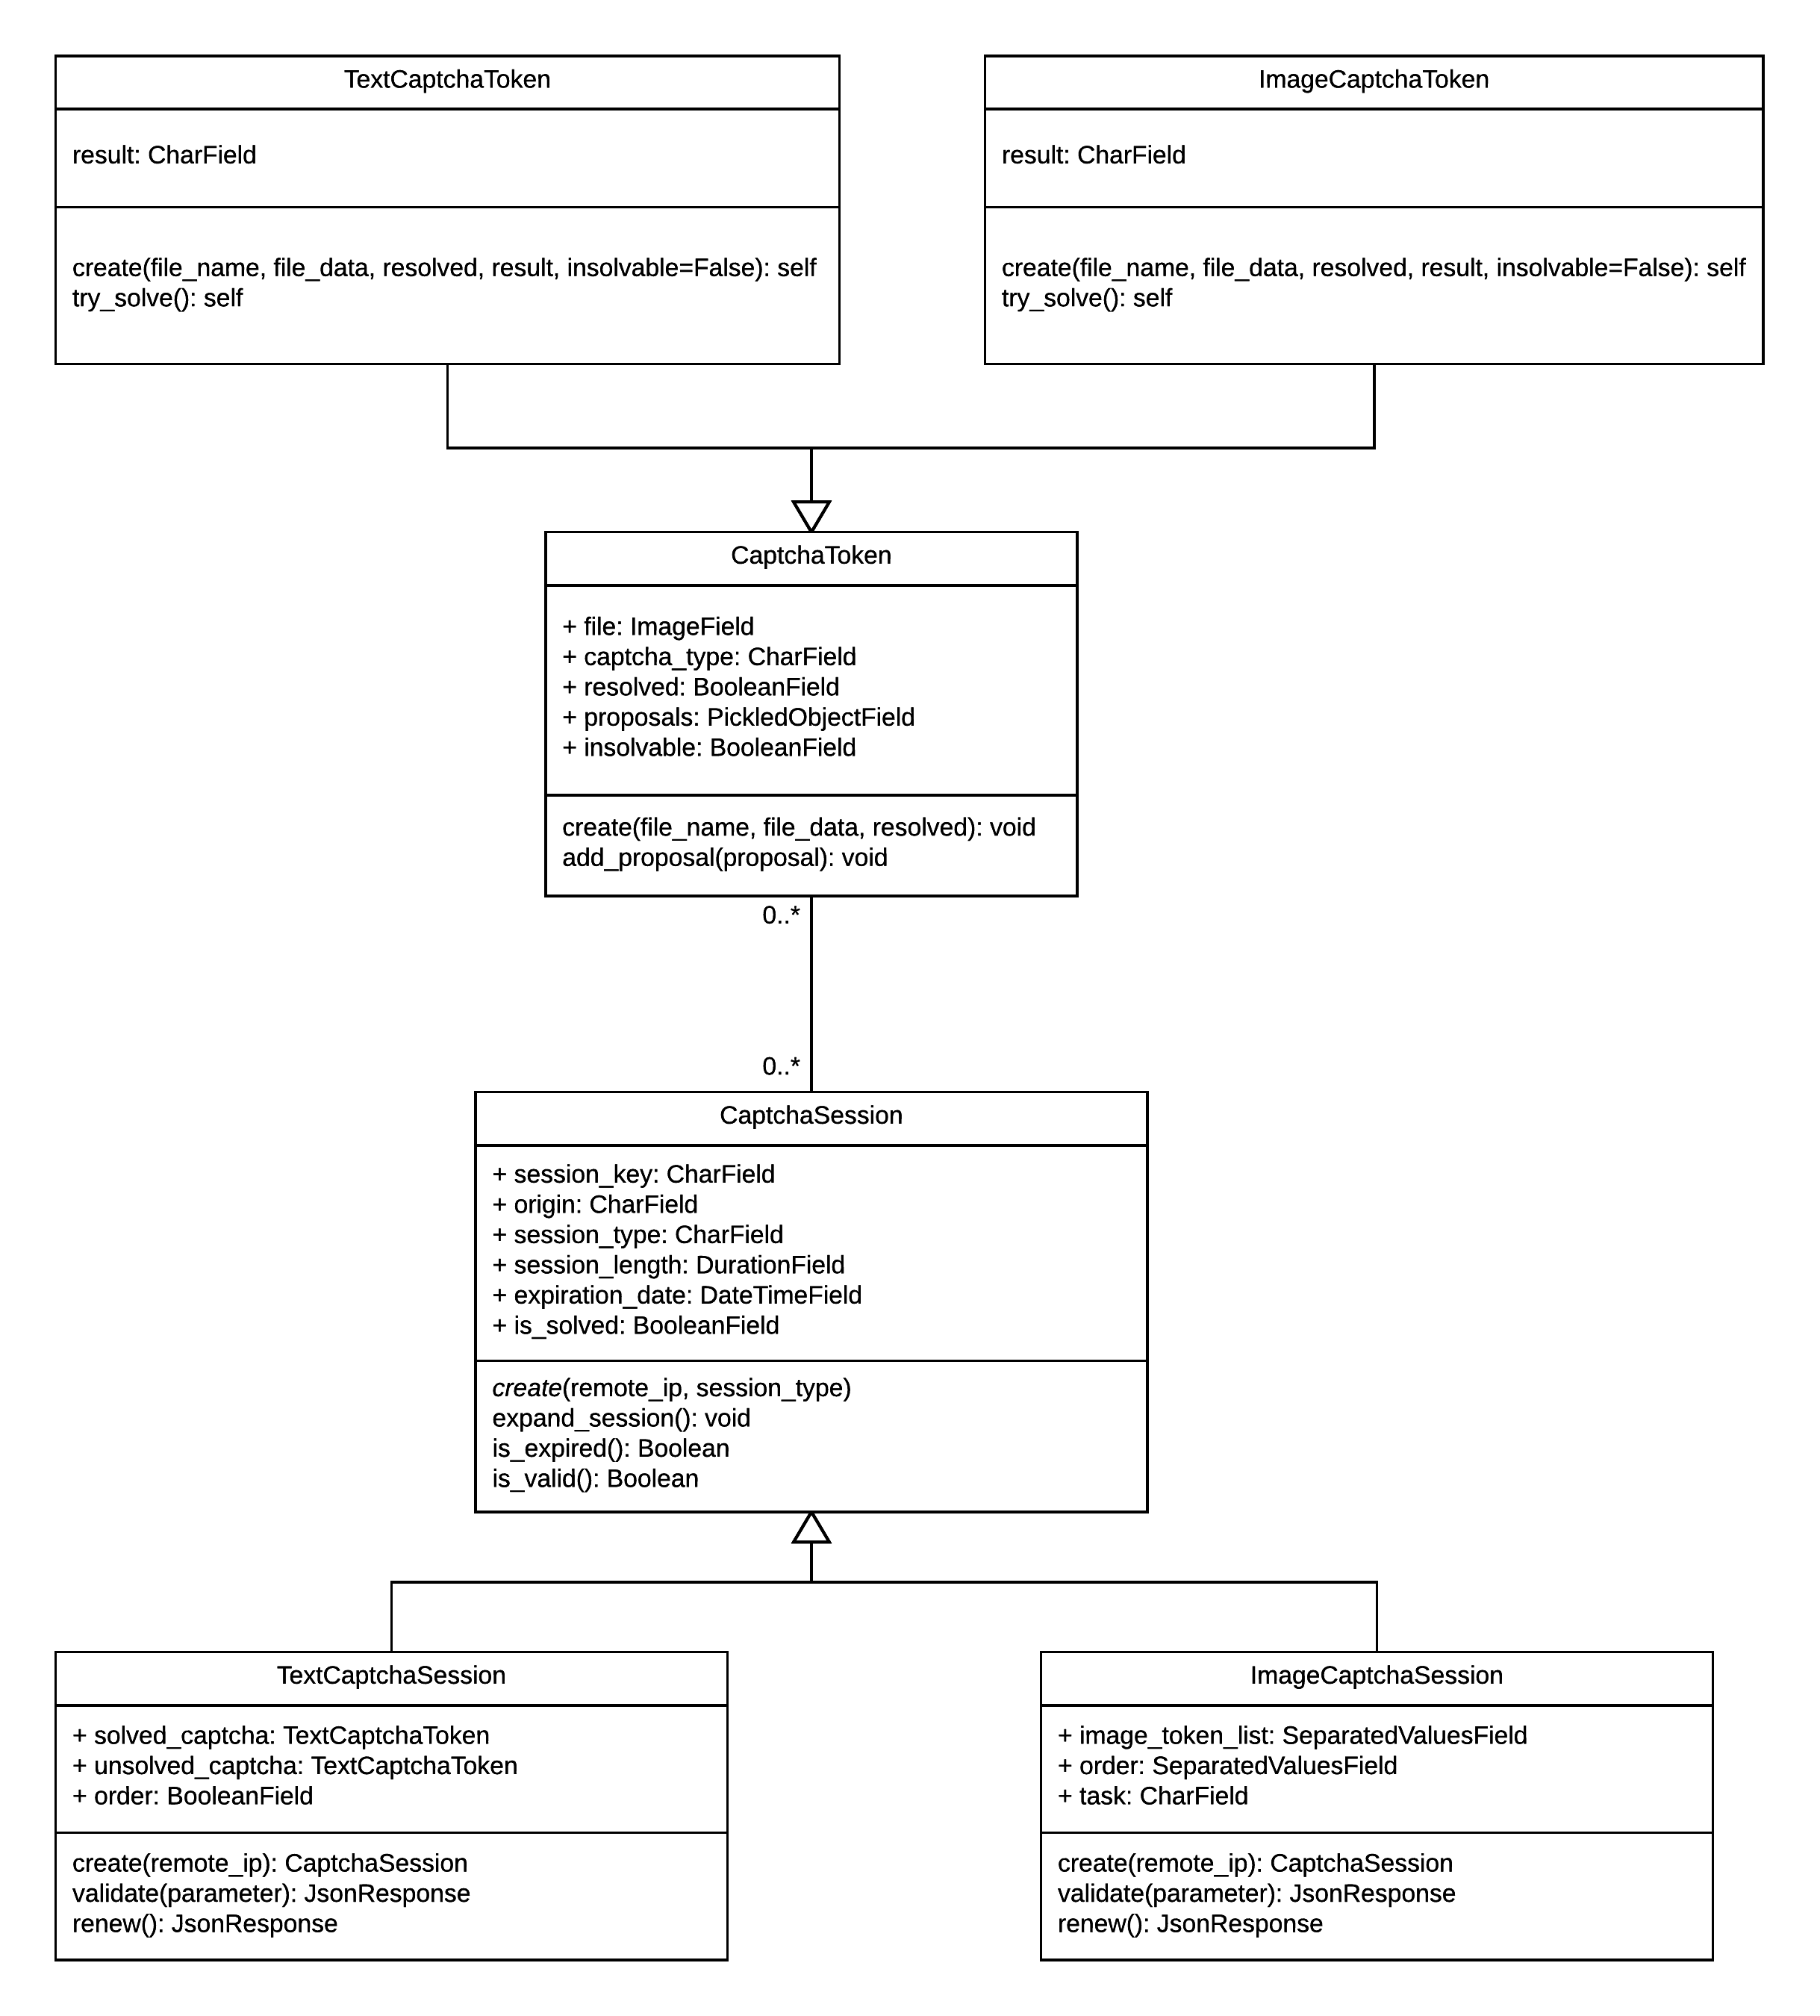
\includegraphics[width=1.1\linewidth]{content/figures/classdiagramm.png}
\caption{Class diagram representing the classes used for the generation of Captchas. The two main classes \emph{CaptchaToken} and \emph{CaptchaSession} are shown in the center. All other classes inherit from one of the superclasses.
}
\label{fig:classdia}
\end{figure}

The class \emph{CaptchaToken} represents a single image, that is part for a Captcha, e.g. a single word, that needs to be written down by the user in order to solve the Captcha. The class \emph{CaptchaSession} represents a complete Captcha challenge a user has to solve, e.g. writing down the words shown on all images. Each type of Captcha challenge provided by the service is represented by a subclass of \emph{CaptchaSession} and \emph{CaptchaToken}. Currently two kinds of Captchas, ImageCaptchas and TextCaptchas, are supported. 


All that needs to be done for implementing a new type of Captcha challenge is to create a new subclass for \emph{CaptchaToken} and \emph{CaptchaSession} and implement specific functionality in these subclasses. Which methods and attributes need to be added in the new subclasses is listed in the ``Attributes and Methods implemented in the subclass''-paragraph.

All instances of a \emph{CaptchaToken} or \emph{CaptchaSession} are saved in the \verb|db.sqlite3|-Database. 

\clearpage
\subsubsection{CaptchaToken}

The class \emph{CaptchaToken} is the basic unit of the Captcha service. Data, which is supposed to be labeled by the Captcha service is saved as a \emph{CaptchaToken}. Multiple \emph{CaptchaTokens} are combined to a Captcha challenge, when a new \emph{CaptchaSession} is created.

\paragraph{Attributes and Methods implemented in the superclass} \mbox{} \\
Attributes:

\begin{itemize}
\item \verb|file|: Image, that is represented by the CaptchaToken.
\item \verb|captcha_type|: String, that defines the type of Captcha the token can be used for. Currently ``text'' for TextCaptchas and ``image'' for ImageCaptchas are supported.
\item \verb|resolved|: Boolean, that indicates, if the solution for a \emph{CaptchaToken} is known or not. A \verb|0| means the token is unsolved and a \verb|1| means the Token is solved.
\item \verb|proposals|: Dictionary, that stores the possible solutions suggested by users of the Captcha service and how often each solution was suggested.
\item \verb|insolvable|: Boolean which indicates, that a token is not solvable by clients of the Captcha service. This value is set to \verb|True|, if there are many proposals for a \emph{CaptchaToken} without one proposal having the majority of the votes. For more information see \hyperref[sec:solving_algorithm]{section 6 (solving algorithm)}.
\end{itemize}

Methods:

\begin{itemize}
\item \verb|create(file_name, file_data, resolved)|: Responsible for basic configuration, that need to be done for all kinds of tokens, when they are created. Only used for super-calls in the \verb|create()|-method of subclasses.
\item \verb|add_proposals(proposal)|: Adds a new suggested solution to the \verb|proposals|-dictionary, or increments the counter for an already suggested proposal.
\end{itemize}

\paragraph{Attributes and Methods implemented in the subclass} \mbox{} \\
Attributes: 

\begin{itemize}
\item \verb|result|: Saves the correct solution for a token. Data type differs between different subclasses, e.g. \emph{TextCaptchaToken} saves a string and \emph{ImageCaptchaToken} saves a boolean.
\end{itemize}

Methods:

\begin{itemize}
\item \verb|create(file_name, file_data, resolved, result, insolvable=False)|: Responsible for configuration of all attributes of the \emph{CaptchaToken}. Returns a \emph{CaptchaToken}.
\item \verb|try_solve|: Responsible for finding the correct solution for a \emph{CaptchaToken} based on the values saved in the \verb|proposals|-attribute.
\end{itemize}

\clearpage
\subsubsection{CaptchaSession}

Represents an instance of a Captcha challenge, that needs to be solved by a certain client. A \emph{CaptchaSession} consists of multiple \emph{CaptchaTokens}, that are chosen randomly in order to create different challenges dynamically. Each Session corresponds to one of the supported types of \emph{CaptchaTokens}. The tokens chosen are a mix of solved and unsolved tokens, in order to make it possible to validate the session and label new data.

\paragraph{Attributes and Methods implemented in the superclass} \mbox{} \\
Attributes:

\begin{itemize}
\item \verb|session_key|: String, that serves as primary key to identify each session. 
\item \verb|origin|: String, that holds the IP address that requested the Captcha challenge. It is used to match requests made by the client to the corresponding session.
\item \verb|session_type|: String, that defines the kind of Captcha challenge, the client has to solve. Currently ``text'' for TextCaptchas and ``image'' for ImageCaptchas are supported.
\item \verb|session_length|: Timedelta, that stores the amount of time in which a session can be validated. The default value is 30 minutes, which is initialised in the \verb|create()| method of \emph{CaptchaSession}.
\item \verb|expiration_date|: Datetime, that stores the date, after which a \emph{CaptchaSession} can not be validated anymore.
\item \verb|is_solved|: Boolean, that stores if a \emph{CaptchaSession} was already solved by the client.
\end{itemize}

Methods:

\begin{itemize} 
\item \verb|create(remote_ip, session_type)|: Responsible for basic creation of a \emph{CaptchaSession} of the requested type for the given IP address. Only used for super-calls in the \verb|create()|-method of subclasses.
\item \verb|expand_session()|: Responsible for changing the \verb|expiration_date| of a \emph{CaptchaSession} so that the session is valid for another \verb|session_length|.
\item \verb|is_expired()|: Responsible for checking, if a session is expired. Returns \verb|True| when the current date is before the \verb|expiration_date|.
\item \verb|is_valid()|: Responsible for checking, if a \emph{CaptchaSession} was successfully validated by a client and is not expired. In that case \verb|True| is returned.
\end{itemize}

\paragraph{Attributes and Methods implemented in the subclass} \mbox{} \\
Attributes:

Each session needs to store the tokens, which were used for creating the session as well as additional information, that is needed for validating the answer given by the client. This can differ for every Captcha type. 

TextCaptchaSession:

\begin{itemize} 
\item \verb|solved_captcha_token|: \emph{TextCaptchaToken}, that is already solved and is used as a control word for the session.
\item \verb|unsolved_captcha_token|: \emph{TextCaptchaToken}, that is not solved and shall be identified by the client.
\item \verb|order|: Boolean indicating the order, in which the two tokens are displayed to the client (0 -> solved, unsolved 1 -> unsolved, solved). It is needed to map the answers given by the client to the right tokens.
\end{itemize}


ImageCaptchaSession:

\begin{itemize}
\item \verb|image_token_list|: List of \emph{ImageCaptchaTokens}, where all tokens used for the session are saved.
\item \verb|order|: List of Booleans, that indicates, which token in the \verb|image_token_list| is solved (0 -> unsolved, 1-> solved).
\item \verb|task|: String, that saves the object that should be detected in the Captcha challenge, e.g. cat, if cats should be identified.
\end{itemize}

Methods: 

\begin{itemize}
\item \verb|create(remote_ip)|: Responsible for creating a \emph{CaptchaSession} and returning the created session to the corresponding \verb|view|, and a JsonResponse with the parameters needed to render the Captcha challenge in the front end (e.g. urls of pictures that are shown in the challenge). Depending on the type of the \emph{CaptchaSession}, the function chooses a mix of multiple \emph{CaptchaTokens} with some of them being unsolved and some of them being solved. The unsolved \emph{CaptchaTokens} are data that shall be labeled and the solved \emph{CaptchaTokens} are used for checking, if the answer for the \emph{CaptchaSession} is correct. 
\item \verb|validate(parameters)|: Responsible for validating the solution for a CaptchaSession and returning the created session to the corresponding \verb|view|. The solution suggested by the client is included in the parameters. The method checks, if the suggested solutions matches the solution for the solved \emph{CaptchaTokens}. If the solution given by the client is correct, \verb|proposals| are added for the unsolved \emph{CaptchaTokens} and \verb|try_solve()| is called on these tokens. If the solution is false new \emph{CaptchaTokens} are chosen for the \emph{CaptchaSession} to prevent brute forcing. Returns a JsonResponse with information, whether the session is valid or not and a list of image-URLs that shall be rendered in the session.
\item \verb|renew()|: Responsible for exchanging the \emph{CaptchaTokens} of a \emph{CaptchaSession}, to create a new challenge or the same session. Returns a JsonResponse of the updated information needed to render the session in the front end.
\end{itemize}

\clearpage
\paragraph{Session length and expiration} \mbox{} \\

A \emph{CaptchaSession} expires after a certain amount of time, in order to prevent replay attacks. For this reason \verb|is_valid()| always returns false after the expiration date is over. The \emph{CaptchaSession} however remains in the database indefintely, because Django does not provide an elegant method to automatically delete session after expiry. Therefore the CaptchaService provides a Django command, which is called \verb|delete_timeouted_sessions| and on execution removes all timed out \emph{CaptchaSessions} in the Database. This can be paired with a cron job so that timed out sessions will be deleted in short intervals. 

\clearpage
\subsection{Views (views.py)}

The views handle POST- and GET-Requests made by the Client, third party web application and the web interface. List of Requests handled by views:

\begin{itemize}
\item \verb|request(request)|: GET-Request called by the client, when a new session is requested. Chooses a type for the session randomly, calls create-Method for the session implemented in \verb|models.py| and directs the response of session.create() to the client.
\item \verb|validate(request)|: POST-Request called by the client, when a solution for a Captcha challenge is submitted. Retrieves the the corresponding \emph{CaptchaSession} from the database, calls the validate-Method of the session and directs the response to the client.
\item \verb|renew(request)|: POST-Request called by the client, when a new challenge for an existing \emph{CaptchaSession} shall be provided. Retrieves the corresponding \emph{CaptchaSession} from the database, calls the renew-Method of the session and directs the response to the client.
\item \verb|upload(request)|: POST-Request called by the web interface, when new files are uploaded to the Captcha service. Extracts the files from the zip-file and creates tokens corresponding to the provided data.
\item \verb|download(request)|: GET-Request called by the web interface, to retrieve tokens and solutions from the database. Collects \emph{CaptchaTokens}, that meet the requirements specified in the web interface, compresses them to a zip-file and returns the file.
\item \verb|getTask(request)|: GET-Request called by the web interface, to get all possible tasks for an \emph{ImageCaptchaSession}. Gets all tasks from the database and returns them as a list in a JsonResponse.
\item \verb|validate_solved_session(request)|: GET-Request called by the third party web application, to check if a \emph{CaptchaSession} was successfully validated by a client. This prevents clients from being able to bypass the Captcha challenge.
\end{itemize}

\clearpage

	\section{Implementation}
\label{sec:implementation}

\subsection{Server Side}
\label{subsec:Server Side}

Lorem ipsum dolor sit amet, consectetur adipiscing elit. In erat mauris, faucibus quis pharetra sit amet, pretium ac libero. Etiam vehicula eleifend bibendum. Morbi gravida metus ut sapien condimentum sodales mollis augue sodales. Vestibulum quis quam at sem placerat aliquet. Curabitur a felis at sapien ullamcorper fermentum. Mauris molestie arcu et lectus iaculis sit amet eleifend eros posuere. Fusce nec porta orci.

\subsection{Client Side}
\label{subsec:Client Side}
The Captcha service integrates seamlessly into existing web applications. It basically works by appending an invisible overlay to the body element of the existing website. The overlay fades in when the user hits the submit button of the captcha protected form. Thereby it does not affect the layout of the existing websites.
\begin{figure}[H]
	\centering
	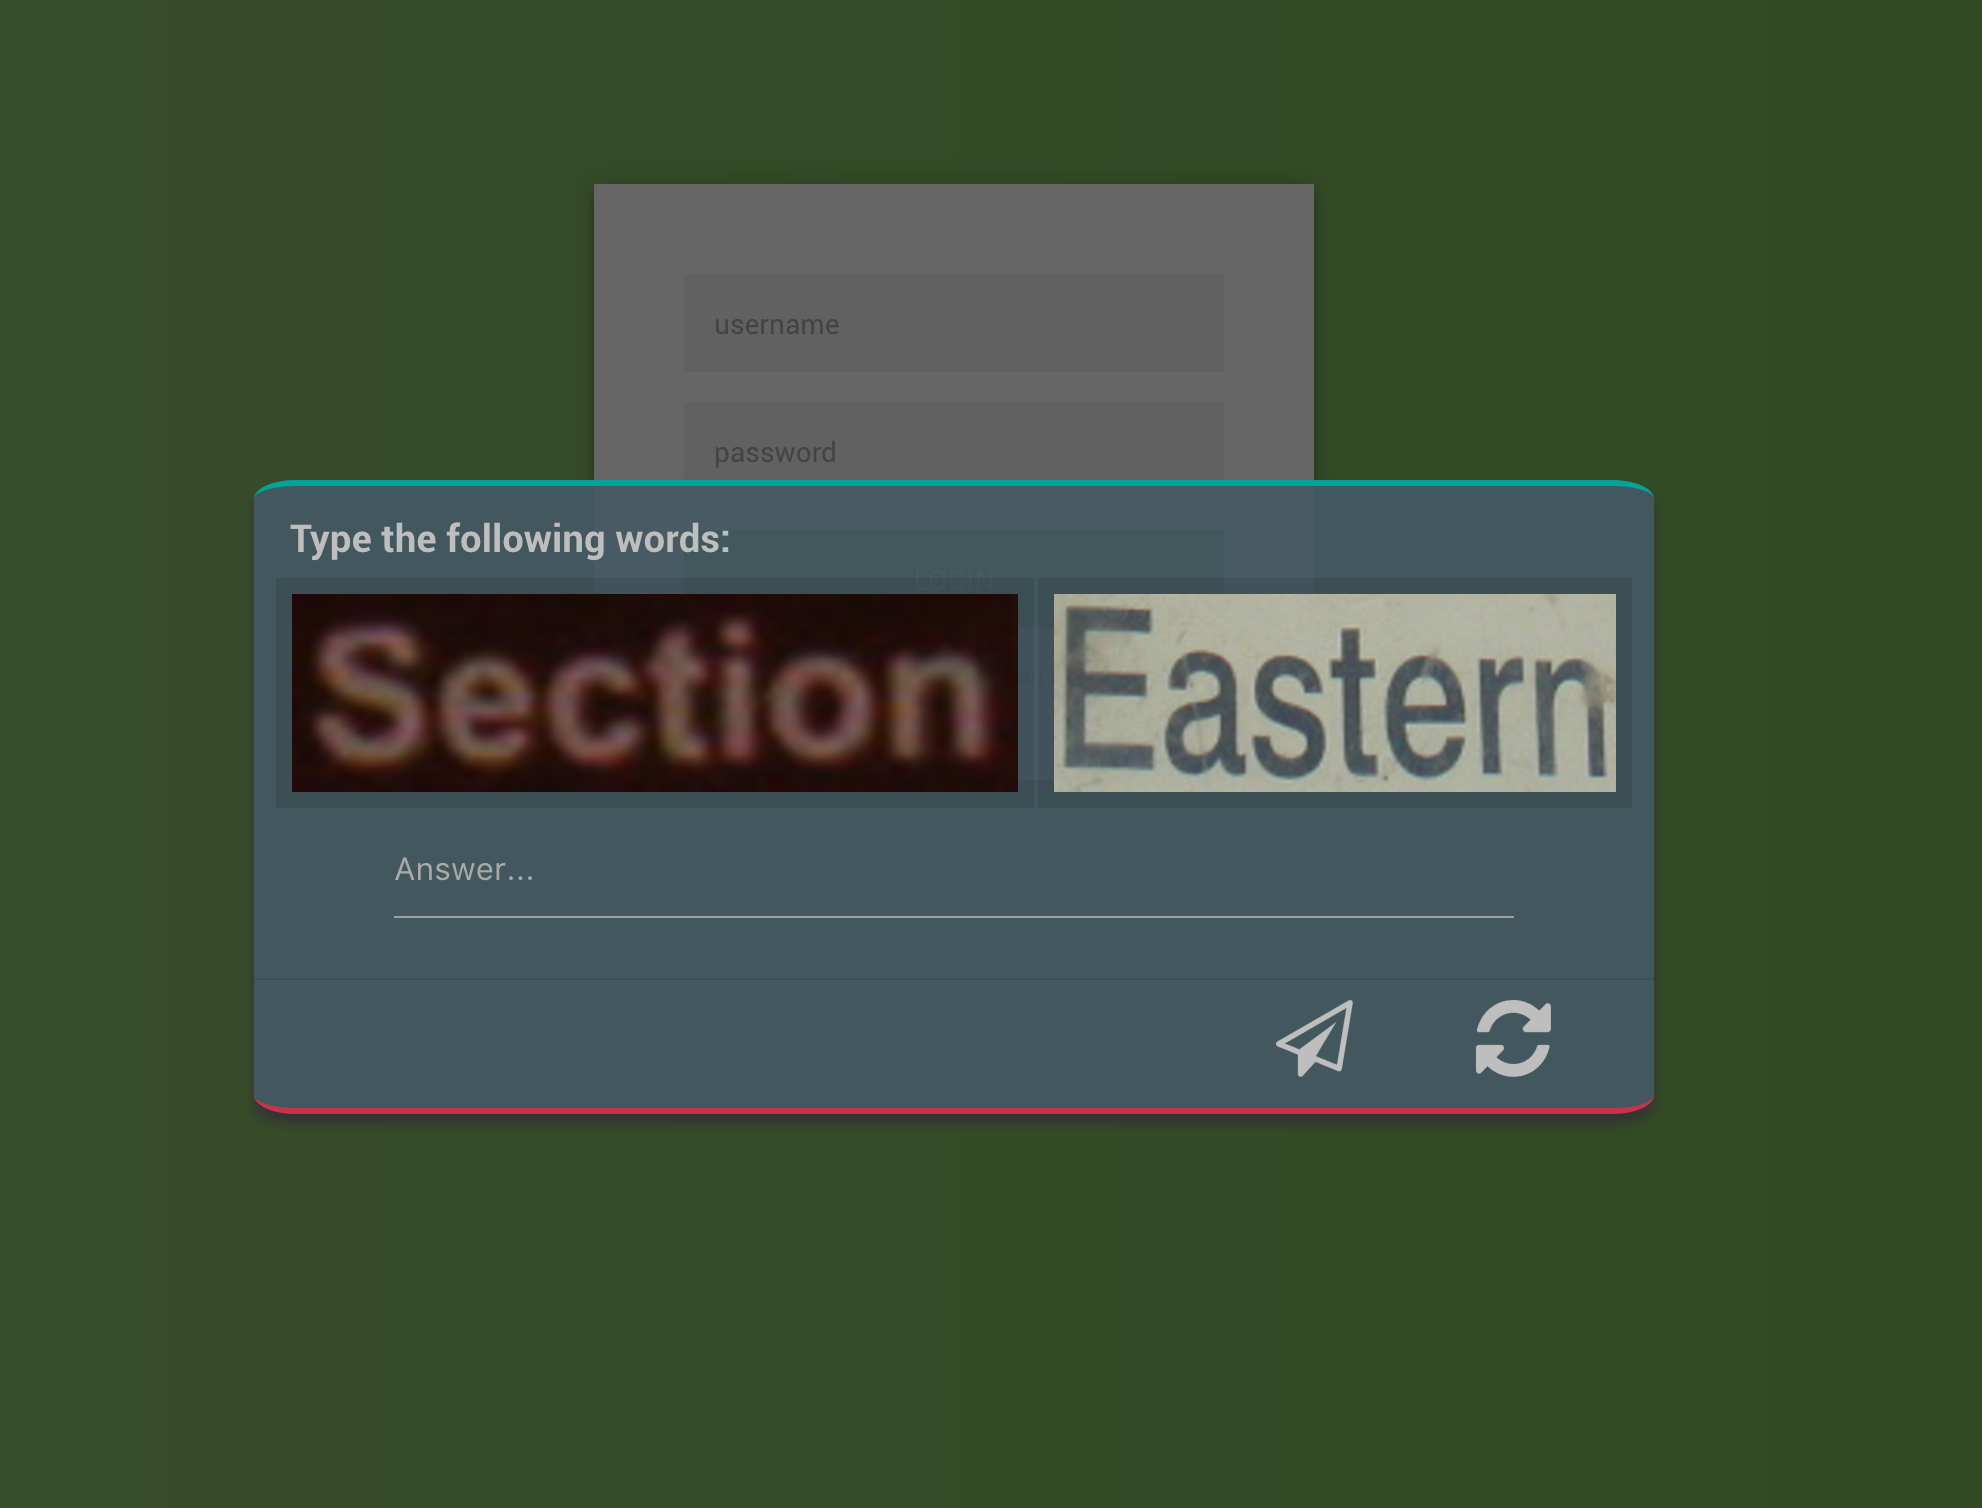
\includegraphics[width=0.8\linewidth]{content/figures/captcha_words.png}
	\caption{Captcha card contents}
	\label{fig:captcha_words}
\end{figure}

 The overlay consists of a \textit{Captcha card}, which in turn consists of a \textit{task}, to be solved \textit{Captcha tokens} and \textit{submit} and \textit{refresh} action elements, as shown in fig. \ref{fig:captcha_words}. As mentioned earlier, we currently support two different Captcha types - namely \textit{text} and \textit{image captchas} - which are randomly delivered to the client. 
 
 \begin{figure}[H]
	\centering
	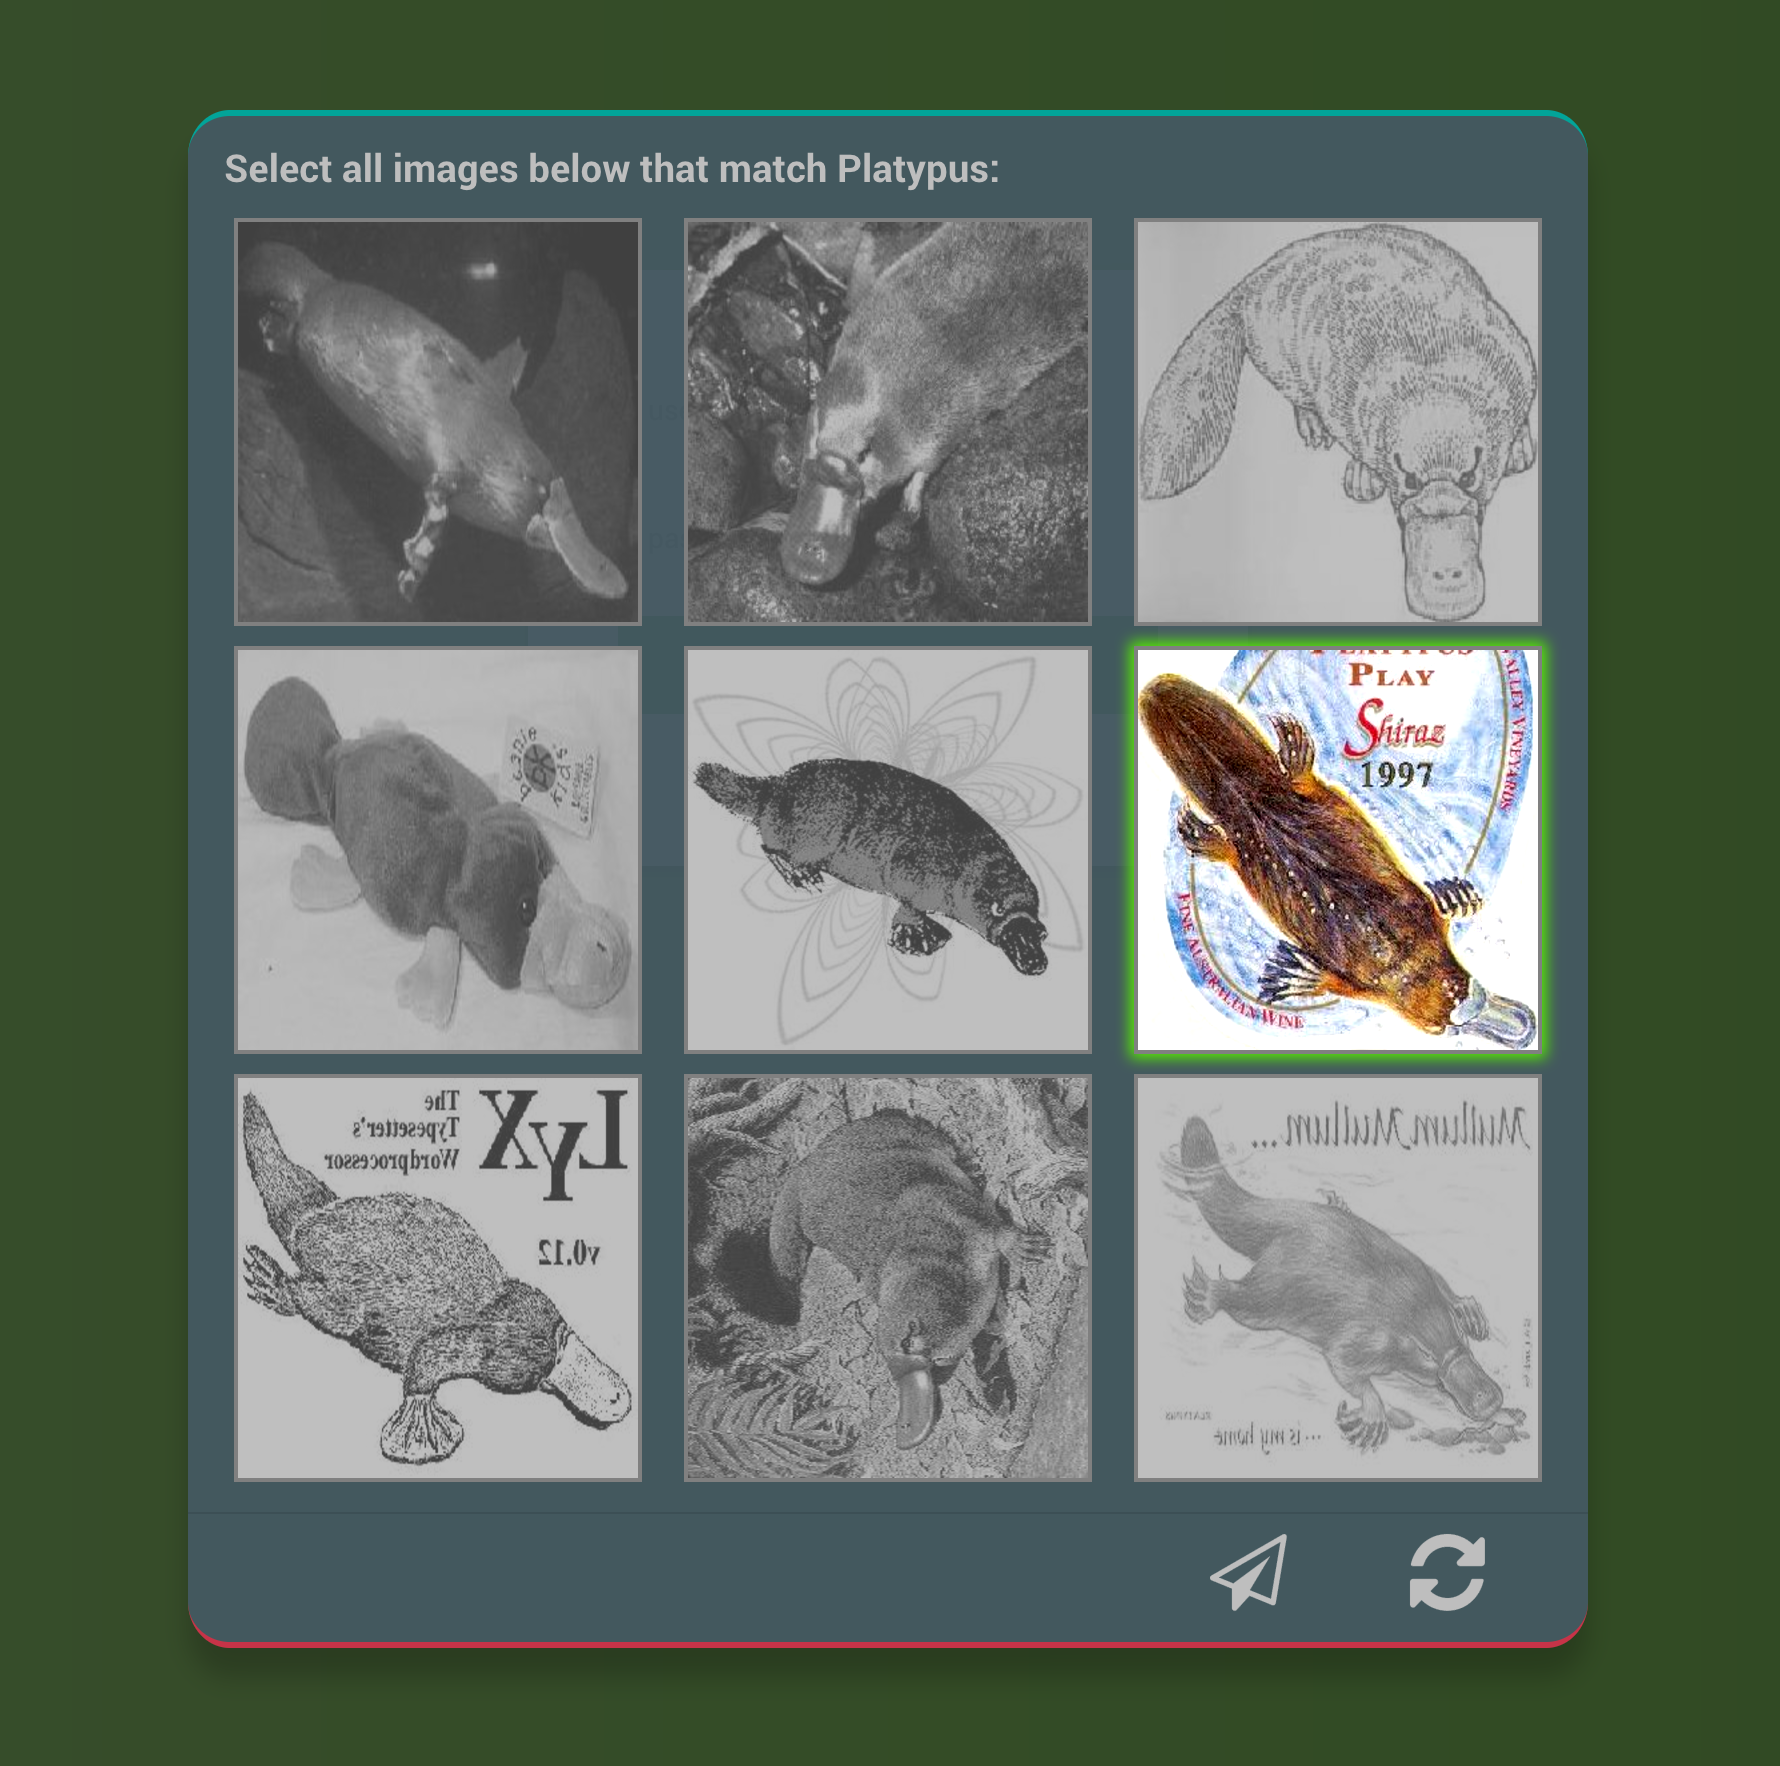
\includegraphics[width=0.8\linewidth]{content/figures/captcha_images.png}
	\caption{Image captcha session}
	\label{fig:captcha_images}
\end{figure}
 
 As soon as the user visits the page, the browser opens a session at the Captcha service via REST API. The browser receives a \textit{session key}, the \textit{Captcha type}, a list of \textit{Captcha tokens} and - in case of an \textit{image Captcha session} - a \textit{task}. The \textit{session key} gets stored in a hidden input field in the Captcha protected form. As a result the \textit{session key} is sent to the web application as soon as the form is submitted, in order to make sure that the client properly solved the Captcha at a later point in time. 
 
 Determined by the \textit{Captcha type} the \textit{Captcha tokens} get either rendered as \textit{text Captcha tokens}, as shown in fig. \ref{fig:captcha_words}, or as \textit{image Captcha grid}, as depicted in fig.\ref{fig:captcha_images}. In case the \textit{session type} is an \textit{image Captcha session}, the task is generated dynamically by inserting the delivered \textit{task} into the HTML, unlike the text Captcha task, which is static.
 
 When the client hits the reload button, the Captcha service is asked via REST API to renew the \textit{session's Captcha tokens}. The response consists of a new list of \textit{tokens} of the same type as before. Subsequently, the old \textit{Captcha tokens} are replaced by the freshly received \textit{Captcha tokens}. The \textit{submit action} triggers the server-side solution validation via REST API. In case the solution was correct the form gets submitted including the \textit{session key}. When the solution is incorrect, the \textit{Captcha card} shakes in order to visually indicate the wrong solution and all newly assigned \textit{Captcha tokens} are inserted. This happens in order to prevent brute force solving. As soon as a wrong solution is submitted, the Captcha service assigns new \textit{Captcha tokens} to the \textit{session} and returns them as response to the client. As a result, you can not restore the old \textit{session tokens} and try to solve it by using all possible inputs.

\subsection{Captcha Integration}
\label{subsec:Captcha Integration}

Integrating the Captcha service into your existing web application is fairly easy. You have to take the following steps:
\begin{enumerate}
	\item inject \texttt{captcha.min.css} and \texttt{captcha.min.js} to your HTML skeleton
	\item  Make sure the to be protected captcha form has the class \textit{captcha-form} and the corresponding submit button possesses the class \textit{captcha-button}
	\item Finally, integrate an additional POST request to our captcha service including the clients \textit{session key} into your existing server-side code, that receives the form data, in order to assure that the user solved the Captcha correctly and did not modify the javascript code.
\end{enumerate}

\texttt{captcha.min.js} includes the client-side code, whose behaviour is described in the last section. \texttt{captcha.min.css} provides the initial styling. Feel free to modify it, such that it fits your design. 

\clearpage

	\section{Image Distortion}
\label{sec:image_distortion}

The fact that images for text captchas are provided by users makes it impossible to tell if those images are easy to recognize for bots and are therefore safe to be used as captcha token. In order to complicate the recognition of the captcha token the systems uses an image distrotion algorithm which is automatically applied to all uploaded text captcha tokens.\\
The image distortion algorithm consists of two steps: the drawing of a horizontal line and a wave transformation. \\
In the first step it places a horizontal line in the middle of the image which is colored with the dominant color of the whole picture. Afterwards this line will be transformed together with the rest of the image.\\
The frequency as well as the amplitude of the wave which will be applied to text are dependent to the height of the image. Furthermore the frequency depends on the width of the image so that one wavelength is at least as wide as the image itself. In addition to this both, the frquency and the amplitude, are modified by a random value in order make every transformation unique. \\
Everything that is shifted out of bounds will be cut off. Additionally the pixels which were located at the bottom and the top of the the original picture will be stretched out vertically to fill the space which was emptied due to the transformation.\\

	\section{Solving Algorithm}
\label{sec:solving_algorithm}

In order to provide a value for the researchers which add data to the captcha service, the system has to label the uploaded images. This becomes possible due to the solving algorithm, which determines the label based on the given user inputs. \\
In case of text captchas the algorithm needs at least three users which solved the captcha correctly. If three or more suggestions match, the image is marked as solved and labeled accordingly. However the token is identified as unsolvable if there are six or more proposals but no more than two of them match. This approach relatively similar to the concept reCaptcha uses. In a paper \footnote{http://science.sciencemag.org/content/321/5895/1465.full} that was published it was stated, that in most cases three human resolutions are enough to label the image reliably. \\
The method for labeling image captchas is similar to the one used for texts. The main difference is the fact that the proposals for these are limited to \textit{true} and \textit{false}, are they suiting the specified task or not. Therefore the algorithm checks if at least four resolutions match and also declares a token as unsolvable if more the six suggestion are given but failed to produces four that match. It was decided to raise the bar for labeling a picture from three to four, because it is more likely to falsely select an image due to a wrong click.
	\section{Evaluation}
\label{sec:evaluation}

As proven by reCAPTCHA, the solving algorithm is accurate most of the time. However, there remains a small chance that images are labeled incorrectly. Certainly there is no way to completely eliminate the possibility of inaccurate labeled images. It would be possible to minimise this probability by further increasing the number of needed proposals, but this would slow the labeling process down and therefore result in fewer labeled images over time. The current implementation provides an acceptable trade-off in order to offer satisfying results for researchers, who rely on this service for data labeling.

Another major feature of the CaptchaService is the ability to reliably combat bots and spammers. The security features, which are in place right now will be enough to hold off the majority of all attacks. However one could argue, that it is not sufficient to renew the Captcha after a wrong proposal and validate the solved session of a user. Further security mechanism, such as blocking of ip addresses after consecutive inaccurate solutions could further increase the security of the system. Nevertheless, it will also worsen the user experience of clients that fail to solve Captchas reliably. This could ultimately lead to users not visiting the website again. Therefore the current implementation does not rely on any further security mechanisms and thus offers an optimal trade-off between user experience an security.

\clearpage

	\section{Future Work}
\label{sec:future_work}

With the thought in mind of building an easy expandable service, the logic consequence would be on focusing on different Captcha types. In the process, key factors such as access for disabled users can be tackled, e.g. by implementing audio Captchas.
Another aspect would be expanding the web interface. The option of downloading solved and unsolved Captchas can be specialized by selecting specific upload times or certain time spans. A feedback of the labeling progress within a task would also be another great tool.



\clearpage
	%%%%%%%%
	
	%%% BIBLIOGRAPHY
	%\bibliographystyle{babunsrt3-fl}
	\addcontentsline{toc}{section}{Bibliography}
	\bibliographystyle{babunsrt-fl}
	\bibliography{projektbib}
	\clearpage	
	
	\appendix
\section{Appendix}
\label{sec:appendix}

Lorem ipsum dolor sit amet, consectetur adipiscing elit. In erat mauris, faucibus quis pharetra sit amet, pretium ac libero. Etiam vehicula eleifend bibendum. Morbi gravida metus ut sapien condimentum sodales mollis augue sodales. Vestibulum quis quam at sem placerat aliquet. Curabitur a felis at sapien ullamcorper fermentum. Mauris molestie arcu et lectus iaculis sit amet eleifend eros posuere. Fusce nec porta orci.

Integer vitae neque odio, a sollicitudin lorem. Aenean orci mauris, tristique luctus fermentum eu, feugiat vel massa. Fusce sem sem, egestas nec vulputate vel, pretium sit amet mi. Fusce ut nisl id risus facilisis euismod. Curabitur et elementum purus. Duis tincidunt fringilla eleifend. Morbi id lorem eu ante adipiscing feugiat. Sed congue erat in enim eleifend dignissim at in nisl. Donec tortor mauris, mollis vel pretium vitae, lacinia nec sapien. Donec erat neque, ullamcorper tincidunt iaculis sit amet, pharetra bibendum ipsum. Nunc mattis risus ac ante consequat nec pulvinar neque molestie. Etiam interdum nunc at metus lacinia non varius erat dignissim. Integer elementum, felis id facilisis vulputate, ipsum tellus venenatis dui, at blandit nibh massa in dolor. Cras a ultricies sapien. Vivamus adipiscing feugiat pharetra.
	
	
\end{document}
